\section{Bridge}

For this section we ventured ahead and built ourself a bridge in minecraft. Importing the bridge into matlab were, apart from some tedious work, quite straight forward.

\subsection{Short overview of algorithm}
Since we wanted to have some kind of time-dependency on our chosen problem, we incorporated a car driving along the bridge. This required us to manually link together the meshes for the bridge and car, and is done in the \it{mergeBridgeCar.m} matlab function. The supplied \it{hex2tetr.m} function is used to split our minecraft cubes into fitting tetrahedrons. We find the boundary points at $z = $, and pass the whole thing into \it{FEM.m} which solves the linear elasticity problem using the finite element method further specified in REF. The function \it{stressRecovery} recovers the nodal Von Mises stresses by averaging the element stresses for each node.



\begin{figure}
\center
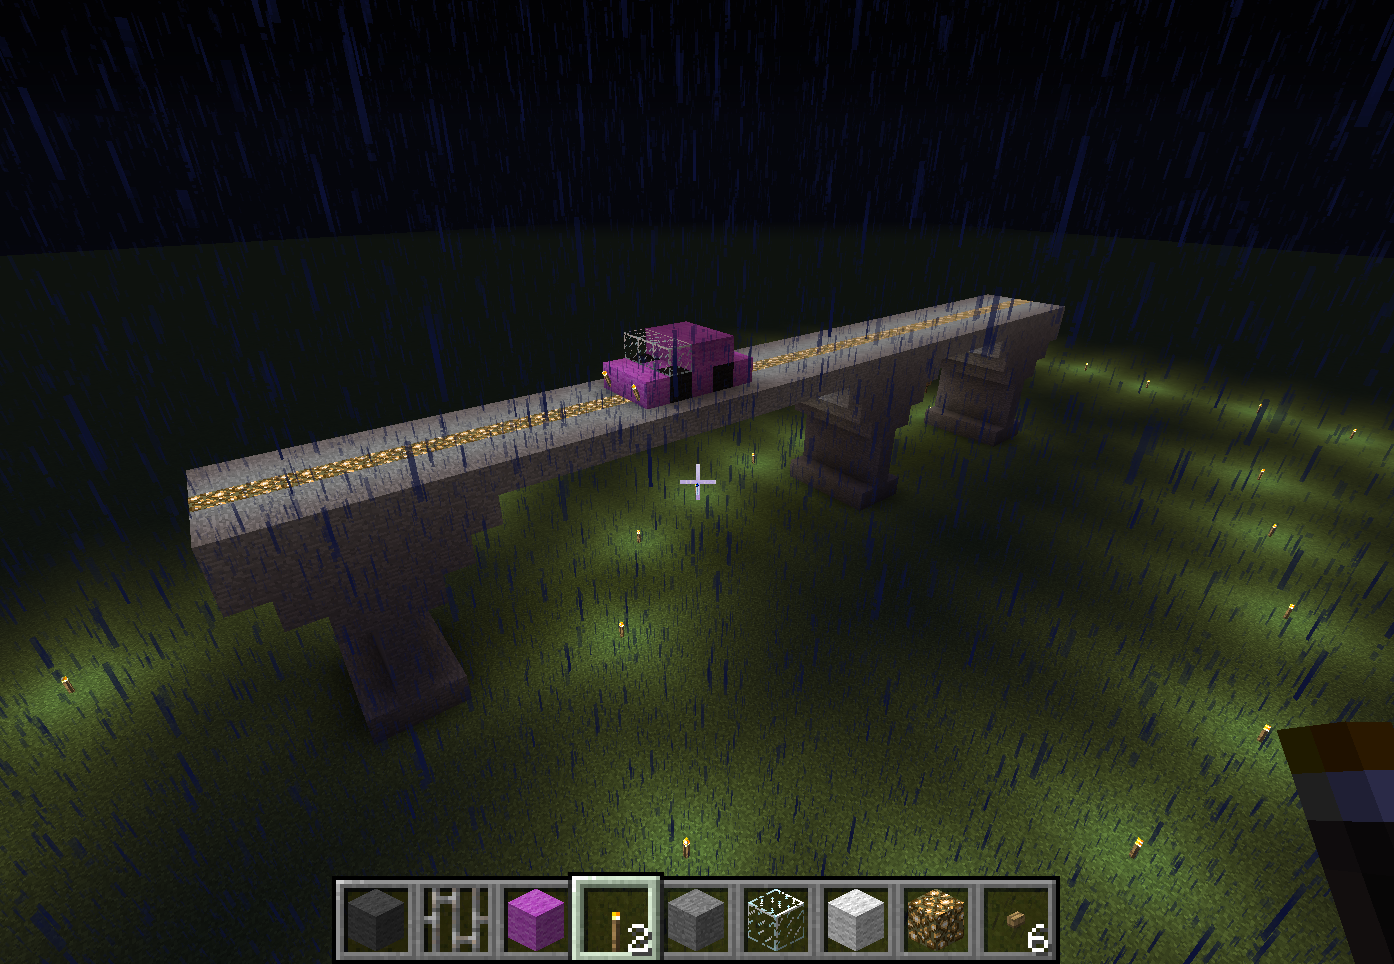
\includegraphics[trim=0cm 5cm 7cm 7cm, clip=true, width=0.9\textwidth]{pic_bridge}
\caption{A picture of the bridge we built in minecraft.}
\label{fig:picBridge}
\end{figure}